\documentclass[letterpaper, 12pt]{article}
\usepackage{hyperref,fancyhdr,lastpage,graphicx,newclude,microtype,}
\usepackage[justification=raggedright,labelfont=bf,format=plain,labelsep=period,textformat=period,singlelinecheck=false]{caption}
\usepackage[margin=1in]{geometry}
\usepackage[T1]{fontenc}
\usepackage[scaled]{helvet}
\renewcommand*\familydefault{\sfdefault}
\setlength{\headheight}{15.2pt}
\pagestyle{fancy}
\rhead[\small{Page \thepage\ of \pageref{LastPage}}]{\small{Page \thepage\ of \pageref{LastPage}}}
\cfoot[\small{Presentation under a Creative Commons license. See the \href{https://github.com/woodrad/Twitter-Sentiment-Mining}{GitHub} project page for information..}]{\small{Presentation under a Creative Commons license. See the \href{https://github.com/woodrad/Twitter-Sentiment-Mining}{GitHub} project page for information.}}
\def\contentsname{}
\usepackage[noae]{Sweave}
\begin{document}

\begin{center}
\huge{\bf{Mining Twitter Using R}}

\normalsize{Presented to the St. Louis R Users Group}

\normalsize{By Mathew Woodyard}

\normalsize{\today}
\end{center}
\hrule
%\tableofcontents

%\newpage

\section{Motivation}
We endevor to answer the questions: Why aren't people buying my widgets? Are people saying bad things about me? Why are the students of Southern Illinois University Edwardsville (\href{http://www.siue.edu/}{SIUE}) unhappy?

These are classic questions concerning not only product marketers, but statisticians. What convinces people to tell us what they think, what they own, what they will buy, where they are, and who they are? How do we get honest answers? What can we infer from a large number of these answers?

There is some good news yet because...

\subsection{300 Million People Are Here To Chat!}
Twitter is a ``microblogging'' service that facilitates communication. Each message, a ``tweet'', contains no more than 140 characters. \href{http://www.wolframalpha.com/input/?i=number%20of%20Twitter%20users}{300 million} people use \href{http://Twitter.com}{Twitter}. But how do they use it? And why? 

Twitter has some use cases and features that result in a nice corpus. Twitter is often used for consumption of news stories and participation in current events. Many people also use twitter to express emotional states: often complaining about and praising places, products, and services. Since tweets contain no more than 140 characters, finding relevant tweets is normally a fairly easy task. Twitter's automatic grouping and ``hashtags'', tags that group topics and start with a hash mark (\#), enable us find what we want with relative ease.

In my example, I will use tweets about SIUE. Tweets were selected from the stream based on the occurrence of the terms ``SIUE'' and ``\#onlyatsiue'', the latter having spent some time as a major regional trending topic.

\begin{figure}[htbp]
\centering

\includegraphics{tweet.png}
\caption{A tweet in its natural habitat}
\end{figure}

Now that we know people are generating data we can use, how can we provide analysis that makes these tweets useful?

\section{Harnessing Tweets}
Our strategy will consist of the following steps.

\begin{enumerate}
\item Sip from the stream of tweets using \href{http://cran.r-project.org/web/packages/twitteR/index.html}{twitteR} and \href{http://cran.r-project.org/web/packages/ROAuth/index.html}{ROAuth} to build a corpus.

\item Discover your new corpus.

\item Select a sentiment lexicon. Download it and load it into R.

\item Score tweets using the function provided or using your own classification scheme.

\item Summarize the results.
\end{enumerate}

\subsection{Building a Corpus}
First, we sip from the stream to build a corpus. Be aware that we can only sip, and not guzzle, due to Twitter's \href{https://dev.twitter.com/docs/rate-limiting}{rate limiting} (note there is no limit on the number of tweets you post using twitteR). The code below loads some previously-downloaded tweets. Code to append new tweets from the stream is commented out and can be ran when you want to expand the corpus. Note that by registering with Twitter's developer program, you can get API keys used to increase the rate limit for your IP/key combination.

\begin{Schunk}
\begin{Sinput}
> # Load needed libraries to allow R to interface with twitter and 
> # interface with the API using OAuth.
> require(twitteR)
> require(ROAuth)
> # The code below does not work due to a current bug in twitteR. 
> # This means that the rate of downloading tweets will be limited.
> # The following code should NEVER be shared. It includes private keys 
> # that authenticate against the twitter API. This code was taken from the 
> # twitteR doccumentation. Run the code from this block to the next comment.
> #
> # reqURL <- "https://api.twitter.com/oauth/request_token"
> # accessURL <- "https://api.twitter.com/oauth/access_token"
> # authURL <- "https://api.twitter.com/oauth/authorize"
> # consumerKey <- "keygoeshere"
> # consumerSecret <- "keygoeshere"
> # twitCred <- OAuthFactory$new(consumerKey=consumer.key,
> #                              consumerSecret=consumer.secret,
> #                              requestURL=reqURL,
> #                              accessURL=accessURL,
> #                              authURL=authURL)
> # twitCred$handshake()
> # 
> # After entering the PIN provided by twitter, run the following command.
> # 
> # registerTwitterOAuth(twitCred)
> 
> # Load saved tweets.
> load(file="../../siue.tweets.RData")
> 
> # Uncomment to add hot new tweets.
> # siueTweets <- append(siue.tweets, searchTwitter('siue', n=1500))
> # siueTweets <- append(siue.tweets, searchTwitter('#onlyatsiue', n=1500))
\end{Sinput}
\end{Schunk}

\subsection{Exploring Your Hot New Corpus}
Now that we have the corpus loaded, let's explore what people from SIUE are saying about their university.

\begin{Schunk}
\begin{Sinput}
> tail(siue.tweets, 2)
\end{Sinput}
\begin{Soutput}
[[1]]
[1] "ktdare: Fire alarm? Check. Short power outage? Check. #onlyatsiue"

[[2]]
[1] "ChrisHeinle2211: thought a goose was going to attack me #OnlyAtSiue"
\end{Soutput}
\end{Schunk}

So far we have some anecdotes and can probably infer that their university had a power outage, is a goose sanctuary, and has a bit of a wasp problem. But what kind of sentiments are associated with SIUE in the aggregate?

\subsection{Loading Lexicons; Preparing Tweets}
Before we can preform more analysis on the aggregate sentements within these tweets, we need to first download and load a sentiment lexicon into R. Then we need to modify the corpus so that we can analyze it.

The Sentiment Lexicon for this project is taken from Hu and Liu's opinion lexicon. See \url{http://www.cs.uic.edu/~liub/FBS/sentiment-analysis.html} for source information and \url{http://www.cs.uic.edu/~liub/FBS/opinion-lexicon-English.rar} to download their opinion lexicon. The raw text is also included in the Git repository for this project.

\begin{Schunk}
\begin{Sinput}
> # Import sentiment lexicons. If the situation demands, 
> # add in domain-specific words.
> positiveWords <- 
+   scan('../../Hu and Liu Sentiment Lexicon/positive-words.txt',
+        what='character', comment.char=';')
> negativeWords <- 
+   scan('../../Hu and Liu Sentiment Lexicon/negative-words.txt',
+        what='character', comment.char=';')
\end{Sinput}
\end{Schunk}

Now we need to restructure the corpus so we can preform the analysis as preformed in this project.

\begin{Schunk}
\begin{Sinput}
> # Extract the text of the tweet for mining.
> tweetText <-lapply(siue.tweets, function(x) x$getText())
> # Remove non-UTF8 characters.
> tweetText <- subset(tweetText, !grepl("[\x80-\xFF]", tweetText))
\end{Sinput}
\end{Schunk}

\subsection{Scoring Tweets}
The function we are using is mainly taken from \href{http://www.slideshare.net/jeffreybreen/r-by-example-mining-twitter-for}{``R by example: mining Twitter for consumer
attitudes towards airlines''} by Jeffrey Breen. If you want to see the function, simply look at the R code in the GitHub project or in the Rnw file that comes with this PDF.

\begin{Schunk}
\begin{Sinput}
> tweetScores <- score.sentiment(tweetText, positiveWords, negativeWords)
\end{Sinput}
\end{Schunk}


\subsection{Summarizing Your Results}
Now we sumarize the results of our mining. This is a pretty simple way to summarize the scores, but it gives the insight that tweets about SIUE from this sample were very slightly positive.
\begin{Schunk}
\begin{Sinput}
> # Summarize and graph histogram with ggplot2.
> summary(tweetScores$score)
\end{Sinput}
\begin{Soutput}
   Min. 1st Qu.  Median    Mean 3rd Qu.    Max. 
-4.0000  0.0000  0.0000  0.1426  0.0000  5.0000 
\end{Soutput}
\end{Schunk}

\begin{figure}[htbp]
\centering
\begin{Schunk}
\begin{Sinput}
> require(ggplot2)
> qplot(score, data=tweetScores, geom="histogram", binwidth=1)
\end{Sinput}
\end{Schunk}
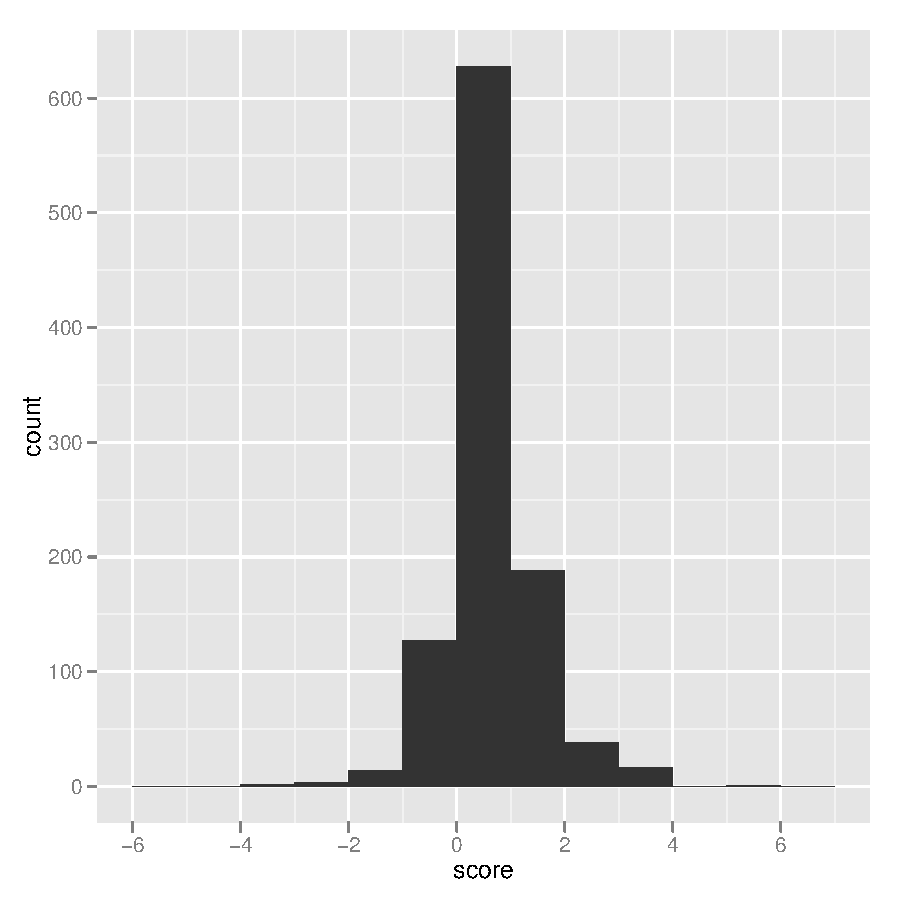
\includegraphics{Handout-008}
\caption{Histogram of tweet scores}
\end{figure}

\section{Limitations}
While we have done lots of stuff, R isn't perfect and this approach is simplistic.

\subsection{Bags of Words Approach}
- Irony and function used. Give example.

\subsection{P\emph{R}oblems}
Problems go here. Like limitations of R and stuff.

\subsection{Requirements}
For thie project, we stand on the shoulders of giants (as always the case when using R). We have received aid and comfort from the packages \verb+plyr+, \verb+stringr+, \verb+twitteR+, \verb+ggplot2+ and \verb+ROAuth+. You will need to have these installed for the code to run. For more information on these packages, see their associated help pages and vignettes.

\section{License}
``Mining Twitter Using R'' by \href{http://5lbs.org}{Mathew Woodyard} is licensed under a \href{http://creativecommons.org/licenses/by-nc-sa/3.0/us/}{Creative Commons Attribution-NonCommercial-ShareAlike 3.0 United States License}. My GitHub project found at \url{https://github.com/woodrad/Twitter-Sentiment-Mining} is under the same license, with the exception of the documentation written by others, which is under the (\href{https://en.wikipedia.org/wiki/Artistic_License}{Artistic}) license listed in the documentation. Permissions beyond the scope of this license may be available at \url{http://5lbs.org}.

\end{document}
